\documentclass{standalone}
\usepackage{chez}

\begin{document}
\chapter{September 28, 2020}

Here is a summary of what we have:
\begin{theorem}[Eilenberg-Steenrod axioms]
  There are functors \(H_n \colon \cTop_2 \to \cAb\). If \(X\) is
  a topological space, we write \(H_n(X) \coloneqq H_n(X, \nullset)\).

  There are natural transformations
  \(\partial \colon H_n(X, A) \to H_{n-1}(A)\) where:
  \begin{itemize}
    \item If \(f_0, f_1 \colon (X, A) \to (Y, B)\) are homotopic, then
      \(H_n(f_0) H_n(f_1)\).
    \item Excisions in \(\cTop_2\) induce isomorphisms on \(H_n\).
    \item For any pair \((X, A)\), the sequence
      \[
        \begin{tikzcd}
          \cdots \ar[r] &
          H_{n+1}(X, A) \ar[r, "\partial"] &
          H_n(A) \ar[r] &
          H_n(X) \ar[r] &
          H_n(X, A) \ar[r, "\partial"] &
          \cdots
        \end{tikzcd}
      \]
      is exact.
    \item \(\displaystyle H_n\parens[\Big]{\smash{\coprod_{i \in I}} X_i}
      = \bigoplus_{i \in I} H_n(X_i)\).
    \item (Dimension axiom) \(H_n(*) = \begin{cases*}
        \ZZ & if \(n = 0\) \\[-1ex] 0 & otherwise.
      \end{cases*}\)
  \end{itemize}
\end{theorem}

An application of excision is that, in favorable conditions,
\(H_n(X, A) \iso H_n(X/A, *) \iso H_n(X, A)\) if \(n > 0\).

\section{Mayer-Vietoris sequence}
One more practical tool for computing the homology of topological spaces is
the \vocab{Mayer-Vietoris sequence}.

Suppose \(X\) is a space and \(\mathcal A = \set{A, B}\) is a cover of \(X\).
Let us label the inclusions
\begin{align*}
  i &\colon A \intersect B \hookrightarrow A \\
  j &\colon A \intersect B \hookrightarrow B \\
  k &\colon A \hookrightarrow X \\
  l &\colon B \hookrightarrow X.
\end{align*}
\begin{theorem}[Mayer-Vietoris]
  There is a long exact sequence
  \[
    \begin{tikzcd}
    	\cdots \ar[r] &
    	H_{n+1}(X) \ar[r, "\partial"] &
    	H_n(A \intersect B) \ar[rr, "H_n(i) \oplus H_n(j)"] &&
    	H_n(A) \oplus H_n(B) \ar[rr, "H_n(k) - H_k(l)"] &&
    	H_n(X) \ar[r, "\partial"] &
    	H_{n-1}(A \intersect B) \ar[r] &
    	\cdots
    \end{tikzcd}
  \]
\end{theorem}
\begin{proof}
  Consider the short exact sequence of chain complexes
  \[
    \begin{tikzcd}
    	0 \ar[r] &
    	S_*(A \intersect B) \ar[rr, "{S_*(i, j)}"] &&
    	S_*(A) \oplus S_*(B) \ar[rr, "S_*(k) - S_*(l)"] &&
    	S_*^{\mathcal A}(X) \ar[r] &
    	0
    \end{tikzcd}
  \]
  By the locality principle, \(H_n(S_*^{\mathcal A}(X)) \iso H_n(X)\),
  so we obtain the Mayer-Vietoris sequence from the long exact sequence
  associated to a short exact sequence of chain complexes.
\end{proof}

\begin{example}
  \begin{minipage}{0.68\textwidth}
    Consider the sphere \(S^2\), with the cover \(\mathcal A = \set{A, B}\),
    where
    \begin{align*}
      A &= \set{(x, y, z) \in \RR^3 \mid z > -1/2}, \\
      B &= \set{(x, y, z) \in \RR^3 \mid z < 1/2},
    \end{align*}
    as in the diagram to the right.
  \end{minipage}
  \begin{minipage}{0.28\textwidth}
    \centering
    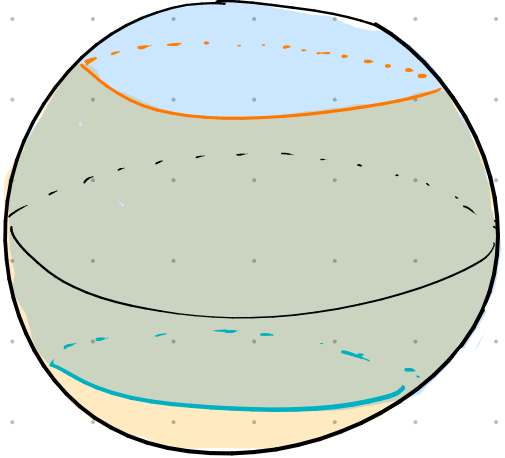
\includegraphics[width=0.55\textwidth]{18_905-200928-1.png}
  \end{minipage}
  \smallskip

  We have the Mayor-Vietoris sequence
  \[
    \begin{tikzcd}
    	H_2(A) \oplus H_2(B) \ar[r] &
    	H_2(S^2) \ar[r, "\partial"] &
    	H_1(A \intersect B) \ar[r] &
    	H_1(A) \oplus H_1(B)
    \end{tikzcd}
  \]
  We know that \(A\) and \(B\) are homotopy equivalent to a point, so
  \(H_2(A) \oplus H_2(B) \iso 0 \oplus 0 \iso 0\).
  Similarly, we know that \(H_1(A) \oplus H_1(B) \iso 0\).
  We also know that
  \(A \intersect B\) is homotopy equivalent to \(S^1\), so
  \(H_1(A \intersect B) = \ZZ\).
  Therefore, the exact sequence is
  \[
    \begin{tikzcd}
    	0 \ar[r] &
    	H_2(S_2) \ar[r, "\partial"] &
    	\ZZ \ar[r] &
    	0
    \end{tikzcd}
  \]
  Exactness says that \(\partial\) is both injective and surjective,
  so \(H_2(S^2) \iso \ZZ\).
\end{example}

\begin{example}
  Let \(T^2 \iso S^1 \times S^1\) be the torus,
  and let \(\mathcal A = \set{A, B}\) be
  the cover as defined by the image:
  \begin{center}
    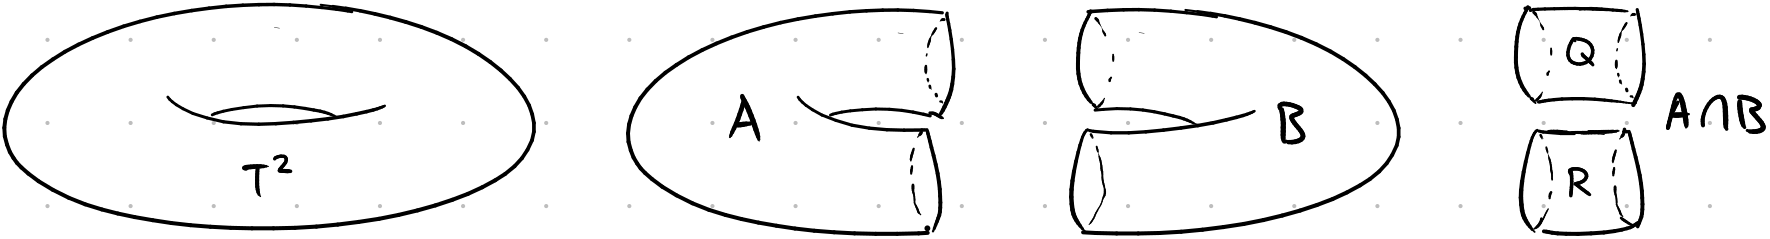
\includegraphics[width=0.8\textwidth]{18_905-200928-2.png}
  \end{center}

  We have the long exact sequence
  \[
    \begin{tikzcd}[column sep=small]
    	H_2(A) \oplus H_2(B) \ar[r] &
    	H_2(T^2) \ar[r, "\partial"] &
    	H_1(A \intersect B) \ar[r] &
    	H_1(A) \oplus H_1(B) \ar[r] &
    	H_1(T^2) \ar[r, "\partial"] &
    	H_0(A \intersect B) \ar[r] &
    	H_0(A) \oplus H_0(B)
    \end{tikzcd}
  \]
  Note that \(A\) and \(B\) are homeomorphic to an annulus,
  and therefore they are homotopy equivalent to \(S^1\).
  This simplifies our sequence to
  \[
    \begin{tikzcd}[column sep=small]
    	0 \ar[r] &
    	H_2(T^2) \ar[r, "\partial"] &
    	H_1(A \intersect B) \ar[r] &
    	\ZZ \oplus \ZZ \ar[r] &
    	H_1(T^2) \ar[r, "\partial"] &
    	H_0(A \intersect B) \ar[r] &
    	\ZZ \oplus \ZZ
    \end{tikzcd}
  \]
  Since \(A \intersect B\) has two path components,
  \(H_0(A \intersect B) = \ZZ \oplus \ZZ\).
  Also, since \(A \intersect B \simeq S^1 \sqcup S^1\),
  we know \(H_1(A) \oplus H_1(B) \iso \ZZ \oplus \ZZ\).
  \[
    \begin{tikzcd}[column sep=small]
    	0 \ar[r] &
    	H_2(T^2) \ar[r, "\partial"] &
    	\ZZ \oplus \ZZ \ar[r] &
    	\ZZ \oplus \ZZ \ar[r] &
    	H_1(T^2) \ar[r, "\partial"] &
    	\ZZ \oplus \ZZ \ar[r] &
    	\ZZ \oplus \ZZ
    \end{tikzcd}
  \]
  This is not enough to understand the homology groups of the torus,
  so we will need to look at some of the maps.
  Consider the map \(g \colon H_0(A \intersect B) \to H_0(A) \oplus H_0(B)\).
  This maps the path component \(Q\), represented by
  \((1, 0) \in \ZZ \oplus \ZZ \iso H_0(A \intersect B)\),
  to \((1, 1)\) because \(Q \subseteq A, B\).
  Similarly \(R \mapsto (1, 1)\).
  Therefore, \(g \colon (x, y) \mapsto (x+y, x+y)\).

  Now consider \(f \colon H_1(A \intersect B) \to H_1(A) \oplus H_1(B)\).
  To think about this, we can consider the natural chain
  \[
    Q \to A \intersect B \to A \sqcup B \to A,
  \]
  and applying \(H_1\) gives
  \[
    \ZZ \to \ZZ \oplus \ZZ \to \ZZ \oplus \ZZ \to \ZZ.
  \]
  This maps \(1 \mapsto (1, 0) \mapsto f(1, 0) \mapsto 1\),
  because \(Q \to A\) is a deformation retract.
  Similarly, \(Q \to B\) is a deformation retract, so \(f(1, 0) = (1, 1)\).
  If we replace \(Q\) with \(R\), we also get \(f(0, 1) = (1, 1)\).
  Therefore, \(f \colon (x, y) \mapsto (x+y, x+y)\).

  This gives the following long exact sequence
  \[
    \begin{tikzcd}[column sep=small, row sep=0.1em]
    	H_2(A) \oplus H_2(B) \ar[r] &
        H_2(T^2) \ar[r] &
        H_1(A \intersect B) \ar[r, "f"] &
        H_1(A) \oplus H_1(B) \ar[r, "r"] &
        H_1(T^2) \ar[r, "s"] &
        H_0(A \intersect B) \ar[r, "g"] &
        H_0(A) \oplus H_0(B) \\
    	0 \oplus H_2(B) \ar[r] &
        H_2(T^2) \ar[r] &
        \ZZ \oplus \ZZ \ar[r] &
        \ZZ \oplus \ZZ \ar[r] &
        H_1(T^2) \ar[r] &
        \ZZ \oplus \ZZ \ar[r] &
        \ZZ \oplus \ZZ \\
    	&
        &
        (x, y) \ar[r, mapsto] &
        (x+y, x+y) &
        &
        (x, y) \ar[r, mapsto] &
        (x+y, x+y)
    \end{tikzcd}
  \]

  Exactness at \(H_2(T^2)\) tells us that
  \(H_2(T^2) \hookrightarrow \ZZ \oplus \ZZ\) is an injection.
  Exactness at \(H_1(A \intersect B) \iso \ZZ \oplus \ZZ\) tells us that
  \(H_2(T) \iso \ker f \iso \ZZ{(1, -1)} \iso \ZZ\).
  Therefore, we have computed \(H_2(T^2) \iso \ZZ\).

  To compute \(H_1(T^2)\),
  note that exactness at \(H_1(A) \oplus H_1(B)\)
  tells us that \(\ker r = \img f \iso \ZZ\),
  and exactness at \(H_0(A \intersect B)\) tells us that
  \(\ker g = \img s \iso \ZZ\).
  Therefore, \(H_1(T^2)/\ZZ \iso \ZZ \implies H_1(T^2) \iso \ZZ \oplus \ZZ\).
\end{example}

\begin{figure}
  \centering
  \begin{tikzpicture}[scale=3]
    \begin{scope}[decoration={markings, mark=at position 0.5 with {\arrow{>}}}]
      \draw[postaction={decorate}] (0, 0) -- (1, 0) node[midway, below]{\(g\)};
      \draw[postaction={decorate}] (0, 1) -- (1, 1) node[midway, above]{\(g\)};
    \end{scope}
    \begin{scope}[decoration={markings, mark=at position 0.5 with {\arrow{>>}}}]
      \draw[postaction={decorate}] (1, 0) -- (1, 1) node[midway, right]{\(f\)};
      \draw[postaction={decorate}] (0, 0) -- (0, 1) node[midway, left ]{\(f\)};
    \end{scope}
    \draw (0, 0) -- (1, 1) node[midway, above left]{\(h\)};

    \node () at (1/4, 3/4) {\(A\)};
    \node () at (3/4, 1/4) {\(B\)};

    \fill (0, 0) circle[radius=0.02];
    \fill (0, 1) circle[radius=0.02];
    \fill (1, 0) circle[radius=0.02];
    \fill (1, 1) circle[radius=0.02];
  \end{tikzpicture}
  \caption{Fundamental polygon of torus}\label{fig:torus-fundamental-polygon}
\end{figure}
A more combinatorial way to think about the torus as a square
with the edges identified like in \cref{fig:torus-fundamental-polygon}.
This represents a semisimplicial set
\[
  \begin{tikzcd}
  	\ZZ\{A, B\} \ar[r] &
  	\ZZ\{f, g, h\} \ar[r] &
  	\ZZ\{x\}
  \end{tikzcd}
\]
which lets us find the homology more combinatorially.
The first map maps \(A \mapsto f + g - h\) and \(B \mapsto g + f - h\).
The second map maps \(f, g, h \mapsto 0\), since all four of the points
are the same.

Our goal in the next few classes is to show that no matter how we cut up
the space.



\end{document}
